\section{Formal Algorithms}\label{app:formal_algorithms}
In this section, we present the algorithms GD and SGD to solve \eqref{GeneralProb}.

\begin{algorithm}[H] 
    \caption{Gradient descent}
    \KwIn{$\mathbf{w}_0 \in \mathbb{R}^p$ as starting point, stepsize $\eta$.}
    \For{k = 0,1,2,...}{
        Set $\mathbf{w}_{k+1} = \mathbf{w}_k - \eta \nabla P(\mathbf{w}_k)$ \\
    }
\end{algorithm}

\begin{algorithm}[H]
    \caption{Stochastic gradient descent}
    \KwIn{$\mathbf{w}_0 \in \mathbb{R}^p$ as starting point, stepsize $\eta$.}
    \For{k = 0,1,2,...}{
        Select $i \in \{1,...,n\}$ uniformly at random. \\
        Set $\mathbf{w}_{k+1} = \mathbf{w}_k - \eta \nabla f_i(\mathbf{w}_k)$ \\
    }
\end{algorithm}

\begin{algorithm}[H]
    \caption{Zeroth order stochastic gradient descent}
    \KwIn{$\mathbf{x}_0 \in \mathbb{R}^p$ as starting point, stepsize $\eta$, and the gradient estimation function $\psi(\cdot,\phi,\mu)$.}
    \For{k = 0,1,2,...}{
        Select $i \in \{1,...,n\}$ uniformly at random. \\
        Set $\hat{\nabla}f_i(\mathbf{x}_k) := \psi(f_i,\mathbf{x}_k,\phi,\mu)$\\
        Set $\mathbf{x}_{k+1} = \mathbf{x}_k - \eta \hat{\nabla}f_i(\mathbf{x}_k)$ \\
    }
\end{algorithm}

\section{Plots of Results}\label{app:plots}
In this section, we present plots that evidence our results in Section~\ref{sec:exp}

\begin{figure}[H]
    \centering
    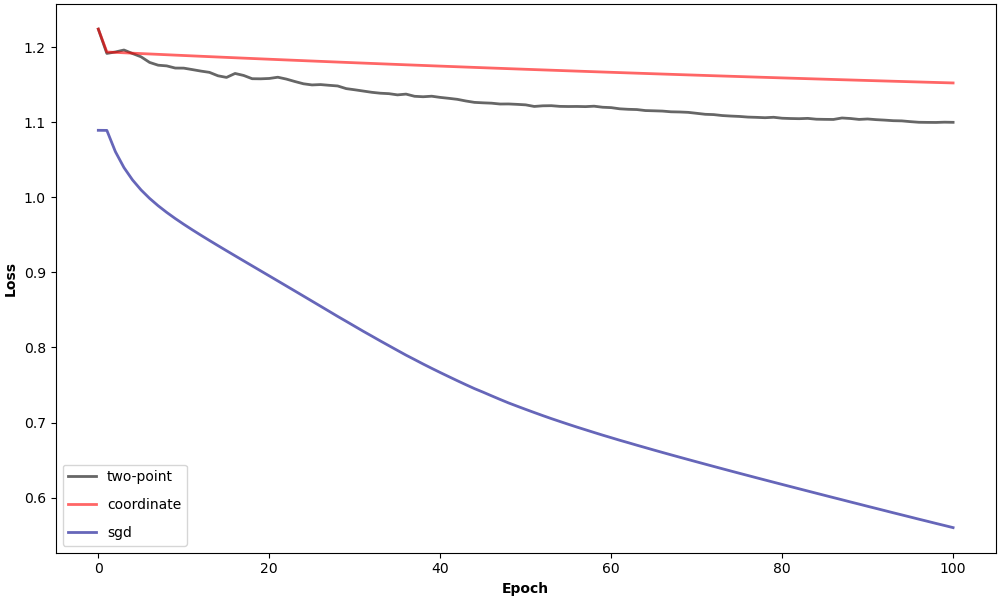
\includegraphics[width=\linewidth]{assets/plot_1.png}
    \label{fig:plot_1}
    \caption{Comparison of loss over epochs of Two-Point and Coordinate Estimation variants of ZO-SGD and SGD with Hidden Dimension $d = 4$ and $\mu = 0.01$. SGD performs better regarding the two other methods over epochs.}
    \label{fig:plot_1}
\end{figure}

\begin{figure}[H]
    \centering
    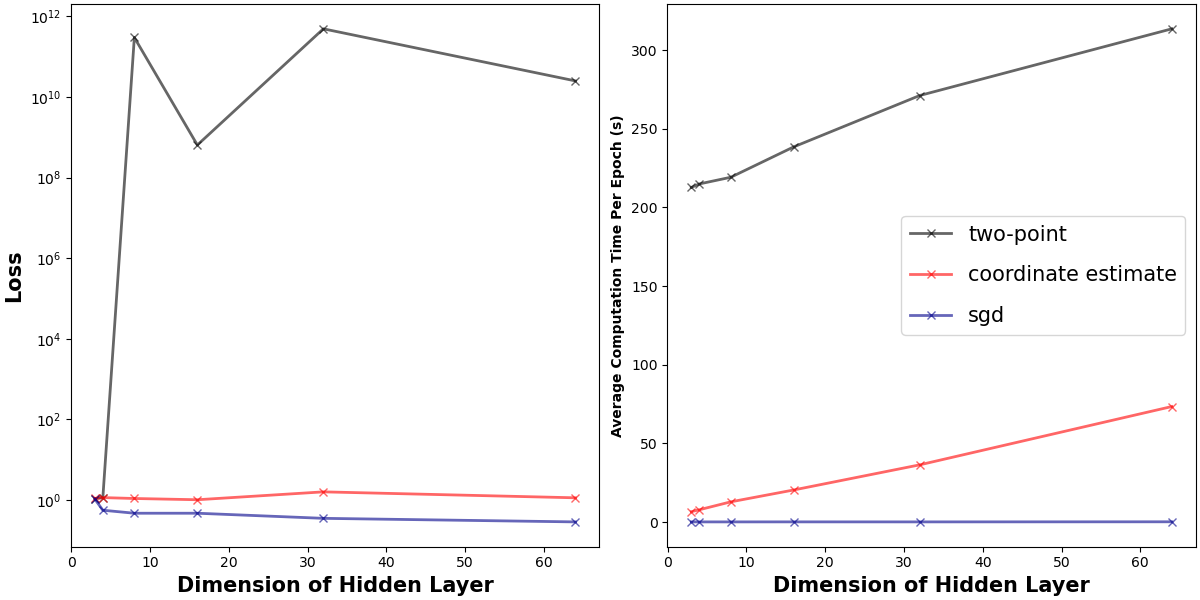
\includegraphics[width=\linewidth]{assets/plot_2.png}
    \caption{Impact of hidden layer dimension on the loss and computational time of two-point and coordinate estimation variants of ZO-SGD and SGD with $\mu = 0.01$. The left plot suggests that two-point estimates are quickly destabilised by high dimensionality, whereas coordinate descent and SGD look robust. The right plot on the other hand shows that the three algorithms scale linearly with dimensionality, but with very different coefficients: dimensionality is more problematic for two-point and coordinate estimates.}
    \label{fig:plot_2}
\end{figure}

\begin{figure}[H]
    \centering
    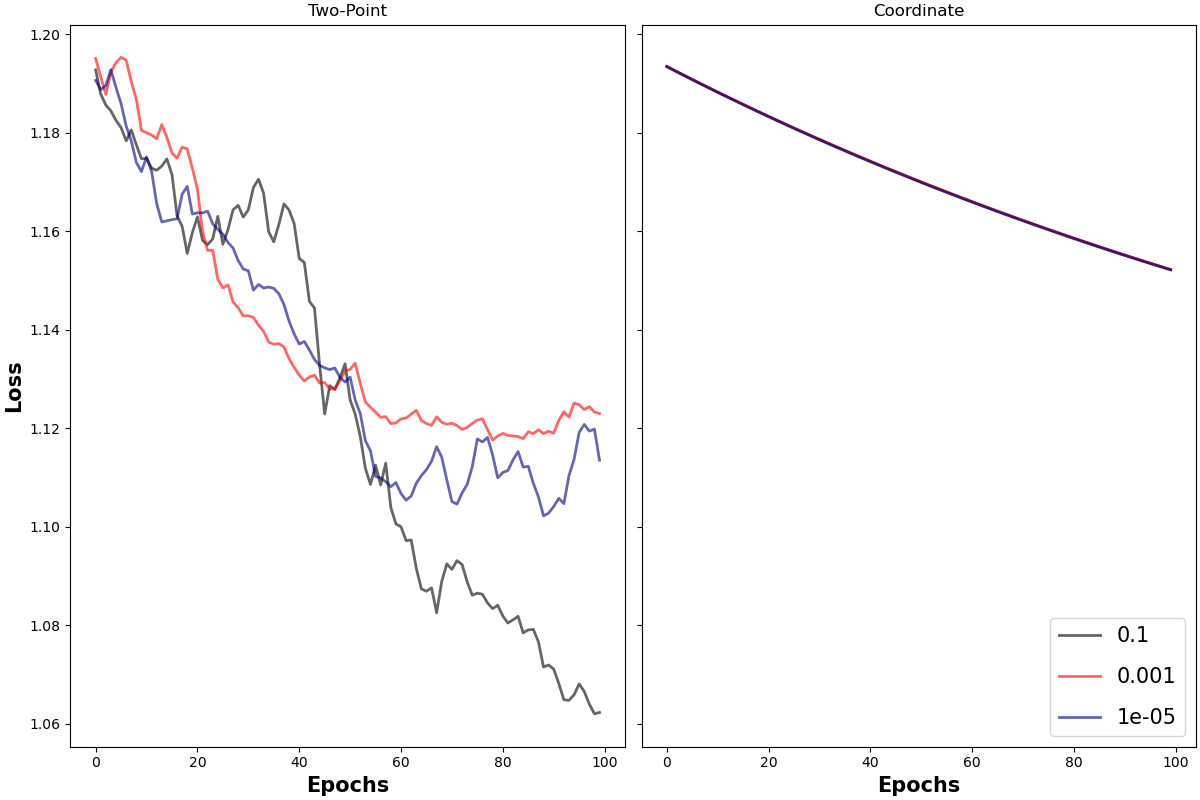
\includegraphics[width=\linewidth]{assets/plot_3.png}
    \caption{Relationship between the perturbation radius $\mu$ and the performance of two-point and coordinate estimation methods for ZO-SGD, varying $\mu$ over $\left\{10^{-1}, 10^{-3}, 10^{-5}\right\}$. The left plot show the loss trajectory of the two-point method, showing small but relatively insignificant changes. The right plot shows the loss trajectory of the coordinate method, showing no noticeable changes. Overall, at these scales, the impact of $\mu$ is minimal.}
    \label{fig:plot_3}
\end{figure}